\documentclass{article}
\usepackage{tikz}
\usetikzlibrary{decorations.pathreplacing}

\begin{document}

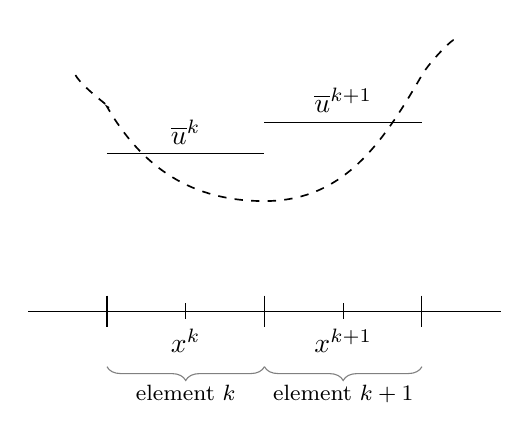
\begin{tikzpicture}[scale=2]

% x-axis
\draw (-1.5,0) -- (1.5,0);
\draw (-1, 0.1) -- (-1, -0.1);
\draw (-0.5, 0.05) -- (-0.5, -0.05) node [below] {$x^k$};
\draw (0, 0.1) -- (0, -0.1);
\draw (0.5, 0.05) -- (0.5, -0.05) node [below] {$x^{k+1}$};
\draw (1, 0.1) -- (1, -0.1);
\draw (-1, 1.0) -- (0, 1.0) node [above,midway] {$\overline{u}^k$};
\draw (0, 1.2) -- (1, 1.2) node [above,midway] {$\overline{u}^{k+1}$};

% line representing function
\draw [dashed, semithick]  
   (-1.2,1.5) to [out=-60,in=330] (-1,1.3)
   to [out=-60,in=180] (0,0.7) 
   to [out=0,in=240] (1,1.5)
   to [out=60,in=60] (1.2,1.7);

\draw [gray,decorate,decoration={brace,amplitude=5pt},yshift=-10pt]
   (1,0) -- (0,0)
   node [black,midway,below=3pt] {\footnotesize element $k+1$};
\draw [gray,decorate,decoration={brace,amplitude=5pt},yshift=-10pt]
   (0,0) -- (-1,0)
   node [black,midway,below=3pt] {\footnotesize element $k$};

\end{tikzpicture}

\end{document}
